\documentclass[border=3pt]{standalone}
\usepackage{tikz}
\usetikzlibrary{arrows.meta,calc,positioning}
\tikzset{pin/.style={-{Stealth[length=5pt]}},
  stage/.style={draw, thick, minimum width=44mm, minimum height=9mm, font=\sffamily\small}}
\begin{document}
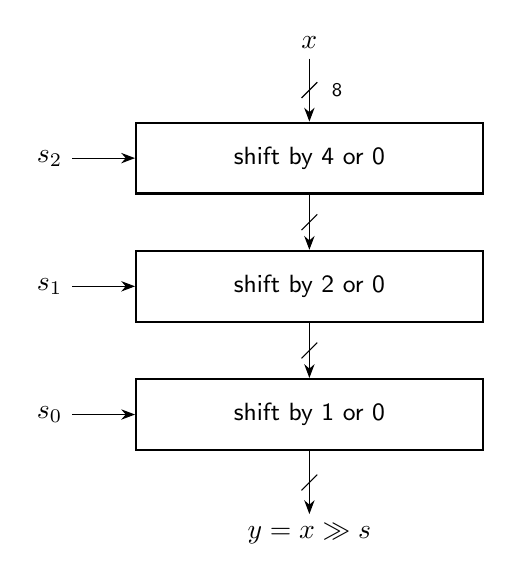
\begin{tikzpicture}[font=\sffamily]
  \node[stage] (s2) at (0,0) {shift by 4 or 0};
  \node[stage, below=7mm of s2] (s1) {shift by 2 or 0};
  \node[stage, below=7mm of s1] (s0) {shift by 1 or 0};
  % data path
  \draw[pin] ($(s2.north)+(0,8mm)$) node[above]{$x$} -- (s2.north);
  \draw[pin] (s2.south) -- (s1.north);
  \draw[pin] (s1.south) -- (s0.north);
  \draw[pin] (s0.south) -- ++(0,-8mm) node[below]{$y = x \gg s$};
  % bus slashes
  \draw ($(s2.north)+(-1mm,3mm)$) -- ($(s2.north)+(1mm,5mm)$);
  \draw ($(s1.north)+(-1mm,2.5mm)$) -- ($(s1.north)+(1mm,4.5mm)$);
  \draw ($(s0.north)+(-1mm,2.5mm)$) -- ($(s0.north)+(1mm,4.5mm)$);
  \draw ($(s0.south)+(-1mm,-5mm)$) -- ($(s0.south)+(1mm,-3mm)$);
  \node[font=\sffamily\scriptsize] at ($(s2.north)+(3.5mm,4mm)$) {8};
  % selects
  \draw[pin] ($(s2.west)+(-8mm,0)$) node[left]{$s_2$} -- (s2.west);
  \draw[pin] ($(s1.west)+(-8mm,0)$) node[left]{$s_1$} -- (s1.west);
  \draw[pin] ($(s0.west)+(-8mm,0)$) node[left]{$s_0$} -- (s0.west);
\end{tikzpicture}
\end{document}
